\documentclass[11pt,a4paper]{article}
\usepackage[utf8]{inputenc}
\usepackage[spanish]{babel}	%Idioma
\usepackage{amsmath}
\usepackage{amsfonts}
\usepackage{amssymb}
\usepackage{graphicx} 	%Añadir imágenes
\usepackage{geometry}	%Ajustar márgenes
\usepackage[export]{adjustbox}[2011/08/13]
\usepackage{float}
\restylefloat{table}
\usepackage[hidelinks]{hyperref}
\usepackage{titling}
\graphicspath{{/home/nazaret/Escritorio/LaTEX}}
%\usepackage{minted}
\usepackage{multirow}
\usepackage{caption}
\usepackage{multicol}
\usepackage[shortlabels]{enumitem}
\usepackage{array}
\selectlanguage{spanish}

%Opciones de encabezado y pie de página:
\usepackage{fancyhdr}
\pagestyle{fancy}
\lhead{Nazaret Román Guerrero}
\rhead{Procesamiento Digital de Señales}
\lfoot{Grado en Ingeniería Informática}
\cfoot{}
\rfoot{\thepage}
\renewcommand{\headrulewidth}{0.4pt}
\renewcommand{\footrulewidth}{0.4pt}

%Opciones de fuente:
\usepackage[utf8]{inputenc}
\usepackage[default]{sourcesanspro}
\usepackage{sourcecodepro}
\usepackage[T1]{fontenc}

\setlength{\parindent}{15pt}
\setlength{\headheight}{15pt}
\setlength{\voffset}{10mm}

% Custom colors
\usepackage{color}
\definecolor{deepblue}{rgb}{0,0,0.5}
\definecolor{deepred}{rgb}{0.6,0,0}
\definecolor{deepgreen}{rgb}{0,0.5,0}

\usepackage{listings}
\usepackage{color}
\usepackage{graphicx}

\definecolor{dkgreen}{rgb}{0,0.6,0}
\definecolor{gray}{rgb}{0.5,0.5,0.5}
\definecolor{mauve}{rgb}{0.58,0,0.82}

\lstset{frame=tb,
  language=python,
  aboveskip=3mm,
  belowskip=3mm,
  showstringspaces=false,
  columns=flexible,
  basicstyle={\small\ttfamily},
  numbers=none,
  numberstyle=\tiny\color{gray},
  keywordstyle=\color{blue},
  commentstyle=\color{dkgreen},
  stringstyle=\color{mauve},
  breaklines=true,
  breakatwhitespace=true,
  tabsize=4
}

\begin{document}
\begin{titlepage}

\begin{minipage}{\textwidth}

\centering

\includegraphics[width=0.5\textwidth]{img/logo.png}\\

\textsc{\Large asignatura\\[0.2cm]}
\textsc{GRADO EN INGENIERÍA INFORMÁTICA}\\[1cm]

{\Huge\bfseries Práctica 2\\}
\noindent\rule[-1ex]{\textwidth}{3pt}\\[3.5ex]
{\large\bfseries Series y Transformada de Fourier. Detección de tonos multifrecuencia}
\end{minipage}

\vspace{1.5cm}
\begin{minipage}{\textwidth}
\centering

\textbf{Autora}\\ {Nazaret Román Guerrero}\\[2.5ex]

\includegraphics[width=0.3\textwidth]{img/etsiit.jpeg}\\[0.1cm]
\vspace{1cm}
\textsc{Escuela Técnica Superior de Ingenierías Informática y de Telecomunicación}\\
\vspace{1cm}
\textsc{Curso 2018-2019}
\end{minipage}
\end{titlepage}

\pagenumbering{gobble}
\pagenumbering{arabic}
\tableofcontents
\thispagestyle{empty}

\newpage

\section{Señales periódicas. Series de Fourier}

Para saber cuáles son los valores que se deben colocar en los generadores de señales de Simulink debemos calcular los valores de $a_0, a_n$ y $b_n$ de la serie de Fourier.

\[x(t)=a_0+ \sum_{n=1}^{\infty} a_n cos(n\omega_0 t) +\sum_{n=1}^{\infty} b_n sin(n\omega_0 t)  \]

Nuestra función es:

\[x(t)=\begin{cases} 
      1 & 0\leq t < T_0/2\\
      -1 & T_0/2 \leq t < T_0
   \end{cases}
\]

Como sabemos que es una señal impar, solo debemos evaluarla entre 0 y $T_0/2$. Vamos a comenzar calculando $a_0$.

\[
	a_0 = \frac{1}{T_0/2} \int_{0}^{T_0/2} x(t)dt  = \frac{1}{T_0/2} \int_{0}^{T_0/2} x(t)dt = \frac{1}{T_0/2}\cdot \int_{0}^{T_0/2}1dt
\]

Resolviendo la integral queda:

\[
	a_0 = \frac{1}{T_0/2}\cdot t\bigg]_{0}^{T_0/2} = \frac{1}{T_0/2}\cdot T_0/2 = 1
\]

Por tanto, $a_0 = 1$.\\

Vamos a calcular ahora $a_n$.

\begin{gather*}
	a_n = \frac{2}{T_0/2}\int_{0}^{T_0/2} x(t)\cdot cos(n\omega_0 t)dt = \\
	= \frac{2}{T_0/2}\int_{0}^{T_0/2} 1\cdot cos(n\omega_0 t) 
	= \frac{2}{T_0/2}\cdot \frac{sin(n\omega_0 t)}{n\omega_0}\bigg]_{0}^{T_0/2} = \\
	= \frac{2}{T_0/2}\left( \frac{sin(n\omega_0\frac{T_0}{2})}{n\omega_0} - \frac{sin 0}{n\omega_0}\right)
	= \frac{2}{T_0/2}\left( \frac{sin(n\omega_0T_0)}{n\omega_0} \right)
\end{gather*}

Por lo tanto sabemos que $a_n =  \frac{2}{T_0/2}\left( \frac{sin(n\omega_0T_0)}{n\omega_0} \right)$. No obstante, puesto que el seno de $\pi$ es 0, el término completo de $a_n$ es 0.\\

Finalmente, vamos a calcular $b_n$, de nuevo entre 0 y $T_0/2$.

\begin{gather*}
	b_n = \frac{2}{T_0/2}\int_{0}^{T_0/2} x(t)\cdot sin(n\omega_0 t)dt = \\
	= \frac{2}{T_0/2}\int_{0}^{T_0/2} 1\cdot sin(n\omega_0 t) 
	= \frac{2}{T_0/2}\cdot \frac{-cos(n\omega_0 t)}{n\omega_0}\bigg]_{0}^{T_0/2} = \\
	= \frac{2}{T_0/2}\left( \frac{-cos(n\omega_0T_0/2)}{n\omega_0} - \frac{-cos 0}{n\omega_0}\right)
	= \frac{2}{T_0/2}\left(\frac{1-cos(n\omega_0T_0/2)}{n\omega_0} \right)
\end{gather*}

Es decir, $b_n = \frac{2}{T_0/2}\left(\frac{1-cos(n\omega_0T_0/2)}{n\omega_0} \right)$.\\

Ahora que tenemos calculados los valores de los tres valores\footnote{Nota para el profesor: No voy a mentir, me he arrepentido mucho de escribir todas las expresiones de arriba en Látex en lugar de escanera el papel, porque es una pesadilla. Pero, ¿a que queda bonito? Queda precioso :D.}, teniendo en cuenta que el período es $\frac{T_0}{2} = \pi$ y $\omega_0 = 2\pi \frac{1}{T_0}$, y que $a_n$ es 0, el desarrollo de la serie es finalmente:


\begin{gather*}
	x(t) = a_0+\sum_{n=1}^{\infty} b_n sin(n\omega_0 t)
	= 1 + \sum_{n=1}^{\infty} \frac{2}{T_0/2} \left(\frac{1-cos(n\omega_0 T_0/2)}{n\omega_0} \right) \cdot sin(n\omega_0 t)
\end{gather*}

Podemos sacar como factor común el factor multiplicativo del segundo término y calcular el valor del coseno que da -1, ya que el coseno de todos los múltiplos de $\pi$ es -1, por lo que el resultado es 2 y podemos sacarlo de la sumatoria. También podemos sacar $\frac{1}{\omega_0}$ como factor común ya que no depende de $n$. Pero $\omega_0=2\pi\cdot f_0=2\pi\cdot \frac{1}{T_0}=2\pi\cdot \frac{1}{2\pi}=1$, por tanto la expresión final es:

\begin{gather*}
	x(t) = 1+ \frac{2}{T_0/2}\sum_{n=1}^{\infty} \left(\frac{1-cos(n T_0/2)}{n} \right) \cdot sin(n t)
	= 1 + \frac{4}{T_0}\cdot 2\sum_{n=1}^{\infty}\frac{sin(nt)}{n} =\\
	= 1+ \frac{4}{2\pi}\cdot 2\sum_{n=1}^{\infty}\frac{sin(nt)}{n} = 1+ \frac{4}{\pi}\sum_{n=1}^{\infty}\frac{sin(nt)}{n}
\end{gather*}

donde vemos que es una sumatoria de senos multiplicada por un factor que es la misma expresión que debíamos demostrar.

\subsection{Valores de frecuencia de los Signal Generator}

Como sabemos, la amplitud se multiplica después de hacer la sumatoria, y es $\frac{4}{\pi}$, que se observa en \texttt{gain4} y \texttt{gain9} en el diagrama de abajo. La frecuencia es lo que se coloca en cada signal generator, y usando la expresión anterior que hemos demostrado, sabemos que las términos donde $n$ es par se van, ya que el seno de los términos pares es 0. Por tanto, solo nos quedamos con los impares: 1, 3, 5, 7... Se puede observar en el diagrama de abajo.

\begin{figure}[H]
	\centering
	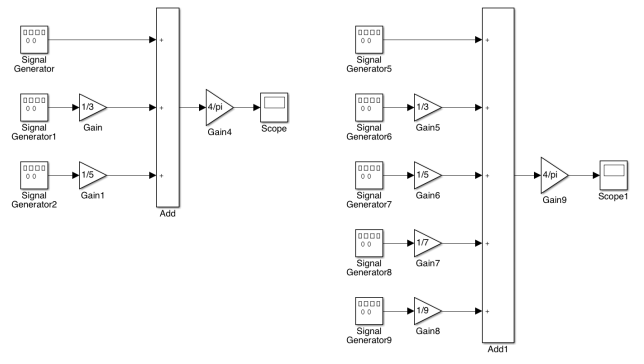
\includegraphics[scale=0.65]{img/simulink.png}
\end{figure}

En la imagen anterior hay dos circuitos distintos. El de la izquierda solo tiene 3 términos por lo que la señal no será  tan fiel a la señal real como lo es el circuito de la derecha. Cuantos más términos se añadan a la sumatoria, más fiel será la representación de la señal generada con la real.

\newpage

\section{Transformada de Fourier de una señal cuadrada}

En este caso, vamos a dibujar una señal cuadrada y su transformada de Fourier. Para ello, tenemos que ejecutar un código (incluido con el nombre de \texttt{signal\_cuadrada.py}) como el que se ve aquí:\\

\begin{lstlisting}
	import numpy as np
	import matplotlib.pyplot as plt
	from scipy.fftpack import fft

	x = np.tile([1,1,1,1,1,1,1,1,-1,-1,-1,-1,-1,-1,-1,-1],64)
	plt.plot(x)

	plt.show()

	X = fft(x)
	f = np.r_[0:0.5:1/1024]
	plt.subplot(1,2,1)
	plt.plot(f,abs(X[0:512]))
	plt.subplot(1,2,2)
	plt.plot(f,np.angle(X[0:512]))

	plt.show()
	\end{lstlisting}

Al ejecutarlo, se nos muestran dos figuras distintas. La primera consta de una única gráfica que se corresponde con la señal original, una señal cuadrada entre 0 y 1000 con una amplitud de entre -1 y 1.

\begin{figure}[H]
	\centering
	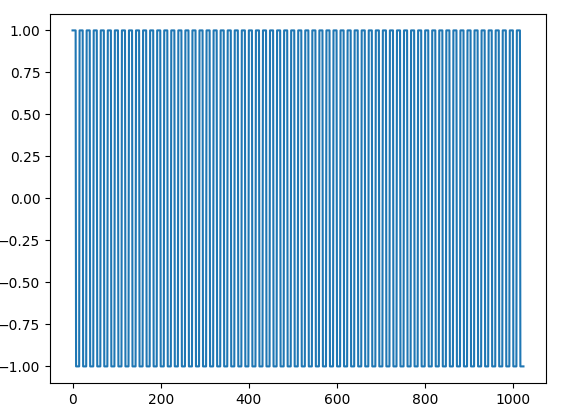
\includegraphics[scale=0.55]{img/signal_cuadrada.png}
\end{figure}

Como se puede observar en el código, después de mostrar esta primera gráfica, se calcula la transformada de Fourier y se muestra la segunda figura; consta de dos gráficas distintas: la primera es la señal tras hacerle la transformada y la segunda es el ángulo de la parte imaginaria de la transformada.

\begin{figure}[H]
	\centering
	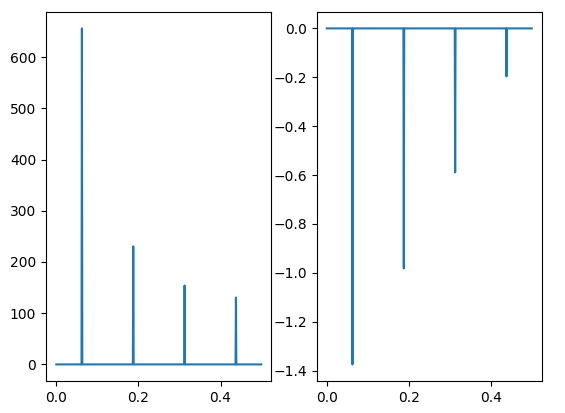
\includegraphics[scale=0.55]{img/signal_fft.png}
\end{figure}

Las dos gráficas de la transformada y el ángulo de la parte imaginaria de la transformada parecen iguales pero invertidas. No obstante, lo que está ocurriendo es que se han cogido muchos valores para simular continuidad en la señal y parece que la transformada no está detectando demasiado bien las variaciones entre ángulos consecutivos.

\newpage

\section{Transformada de Fourier en señales muestreadas}

En este caso, vamos a utilizar una transformada de Fourier para las señales muestreadas y después la compararémos con la transformada de Fourier implementada en el paquete \texttt{numpy} de python.\\

El código para la función es el siguiente:

\begin{lstlisting}
import numpy as np
import matplotlib.pyplot as plt

def fft_senial_muestreada(x):
	# Calculamos la longitud de la muestra
    N = len(x)
    
    # Calculamos la expresion para poder calcular la sumatoria
    W = np.exp(-1j*2*np.pi/N)
    
    # Array donde almacenaremos los resultados inicializado a 0
    X = [0]*N

    for k in range(N):
        for j in range(N):
            X[k] = X[k]+x[j]*(W**(k*j))
            
        # Debemos filtrar un poco y poner los valores muy bajos a 0, ya que de lo contrario tiene mucha sensibilidad y la grafica del angulo de la parte imaginaria da saltos
        if X[k] < 10 ** -5:
            X[k] = 0.0

	# Eliminamos los parentesis del array para que matplotlib pueda leerlo
    X = np.array(X).ravel()

    return X
\end{lstlisting}

Al ejecutar el programa (el archivo está en el \texttt{.zip} bajo el nombre de \texttt{transformada\_fourier.py})
la salida es la siguiente:

\begin{figure}[H]
	\centering
	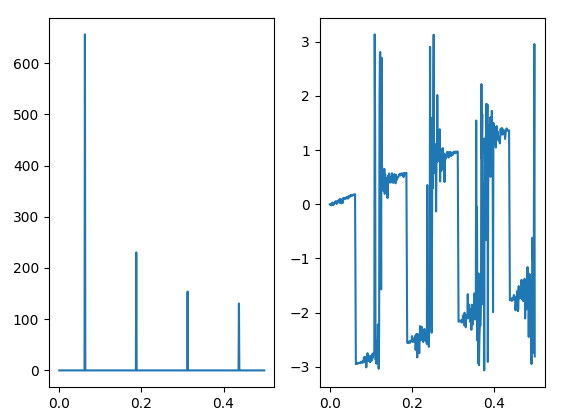
\includegraphics[scale=0.55]{img/mi_fft.png}
\end{figure}

Como se puede observar, la señal que hemos conseguido es igual a la que implementa python, así que hemos creado una transformada de Fourier para señales muestreadas.

\newpage

\section{Detección de tonos multifrecuencia}

En este último apartado vamos a crear un detector de tonos multifrecuencia.\\

Cuando llamamos a una compañía telefónica nos piden marcar números según lo que deseamos. Para saber qué número ha sido marcado se utiliza la detección de las frecuencias que componen esa tecla.
El código está explicado para que se entienda lo que se ha hecho. Utilizando el audio incluido en la práctica, \texttt{digitos.wav}, la salida con un cierto margen de error es *59*256887.\\

El código es el siguiente (también está incluido en el \texttt{.zip} con el nombre de\\ \texttt{tonos\_multifrecuencia.py}):

\begin{lstlisting}
import numpy as np
from scipy.io import wavfile

# Creamos un diccionario con la combinacion de las frecuencias para sacar el digito se ha pulsado
dtmf = {(697, 1209): "1", (697, 1336): "2", (697, 1477): "3", (770, 1209): "4", (770, 1336): "5", (770, 1477): "6", (852, 1209): "7", (852, 1336): "8", (852, 1477): "9", (941, 1209): "*", (941, 1336): "0", (941, 1477): "#", (697, 1633): "A", (770, 1633): "B", (852, 1633): "C", (941, 1633): "D"}

# Leemos el fichero y sacamos la frecuencia y los tonos del audio
Fs, s = wavfile.read('digitos.wav')

# Necesitamos establecer la precision puesto que de lo contrario el toma los valores erroneos del audio debido al ruido de fondo
precision = 0.065
duracion = len(s)/Fs

# Calculamos el desplazamiento segun la duracion del audio y la precision que hemos tenido que establecer y nos quedamos con la parte entera (operador //)
desplaz = int(len(s)//(duracion//precision))

# Vamos a extraer los tonos. Para ello, recorremos toda la informacion dando saltos de tam desplaz
for i in range(0, len(s)-desplaz, desplaz):
    r = s[i:i+desplaz]

    # Calculamos las frecuencias a las que debemos calcular la transformada. Los saltos se producen segun el desplazamiento que hemos declarado antes. Ademas calculamos las frecuencias para asignarlas a las teclas
    Y = np.fft.fft(r)
    frecuencias = np.fft.fftfreq(r.size, d=1/Fs)

    # Frecuencias bajas. Establecemos el minimo y el maximo
    inicio = np.where(frecuencias > 0)[0][0]
    fin = np.where(frecuencias > 1000)[0][0]

    # Extraemos el pico segun la amplitud de la onda. Ese pico se corresponde con el tono de la tecla que hemos marcada
    freq = frecuencias[inicio:fin]
    amplitud = abs(Y.real[inicio:fin])

    # Cogemos el peor valor como el inicial y a partir de este buscaremos uno mejor. Para ello tomamos la frecuencia con mayor amplitud
    freq_baja = freq[np.where(amplitud == max(amplitud))[0][0]]

    # Necesitamos establecer una precision porque de lo contrario coge el ruido como sonidos provocados por una tecla
    diferencia = 10
    mejor = 0

    # Buscamos la frecuencia que tenga una menor diferencia con la frecuencia ideal, utilizamos diferencia como pivote para calcular el mejor tono. Cada vez que encontramos uno mejor, actualizamos la diferencia
    for f in [697, 770, 852, 941]:
        if abs(freq_baja-f) < diferencia :
            diferencia = abs(freq_baja-f)
            mejor = f

    # Nos quedamos con la mejor
    freq_baja = mejor

    # Ahora buscamos la frecuencia alta, igual que hemos hecho con la baja
    inicio = np.where(frecuencias > 1000)[0][0]
    fin = np.where(frecuencias > 1700)[0][0]

    freq = frecuencias[inicio:fin]
    amplitud = abs(Y.real[inicio:fin])

    freq_alta = freq[np.where(amplitud == max(amplitud))[0][0]]

    diferencia = 10
    mejor = 0

    # Buscamos la frecuencia mas alta del tono que estamos tratando
    for f in [1209, 1336, 1477, 1633] :
        if abs(freq_alta-f) < diferencia :
            diferencia = abs(freq_alta-f)
            mejor = f

    freq_alta = mejor

    # Si  no encontramos ningun tono que tenga una frecuencia alta o baja que este por debajo del umbral de precision que hemos impuesto no lo consideramos y no lo codificamos como una tecla
    if freq_baja == 0 or freq_alta == 0:
        c = ""

    # En otro caso, mostramos el caracter que se corresponde con las frecuencias que hemos calculado
    elif dtmf[(freq_baja,freq_alta)] != c:
        c = dtmf[(freq_baja,freq_alta)]
        print(c, end='', flush=True)

\end{lstlisting}

El código está explicado línea por línea, así que ahora lo voy a explicar algo más general para que se entienda la idea.\\

Como sabemos qué frecuencias alta y baja corresponde a cada dígito, creamos una tabla que después usaremos para extraer el número marcado. Leémos el fichero y establecemos una precisión (cuanto más alta sea la precisión más filtra, yo he establecido 0.065 porque de lo contrario solo detectaba los tonos con una frecuencia más alta, por lo que números como el 2 no los reconocía).\\

Recorremos el array con las frecuencias en saltos de \texttt{desplaz} en \texttt{desplaz}. El tamaño de desplazamiento elegido depende del número de muestras y la duración del audio, pero también de la precisión con la que filtramos: cuanto mayor sea la precisión, más saltos serán necesarios puesto que la ventana de desplazamiento abarcará menos valores en una vuelta del bucle para intentar tomarlos de manera más precisa.\\

Con las frecuencias que hemos extraído, calculamos su transformada de Fourier. Una vez las tenemos, buscamos las frecuencias bajas y altas; para ello, establecemos un margen de diferencia con la frecuencia ideal (un delta) y vamos comparando las frecuencias que hemos calculado con la transformada. Cuando encontramos una que tiene mejor delta que la anterior (una diferencia menor con la frecuencia ideal), la tomamos como la mejor hasta el momento.\\

Una vez que hemos calculado la mejor para cada carácter, las buscamos en la tabla que habíamos hecho al principio dándonos finalmente el resultado: *59*256887.

\end{document}